%%%%%%%%%%%%%%%%%%%%%%%%%%%%%%%%%%%%%
\section{Design}
%%%%%%%%%%%%%%%%%%%%%%%%%%%%%%%%%%%%%
\begin{figure}[t]
\centering
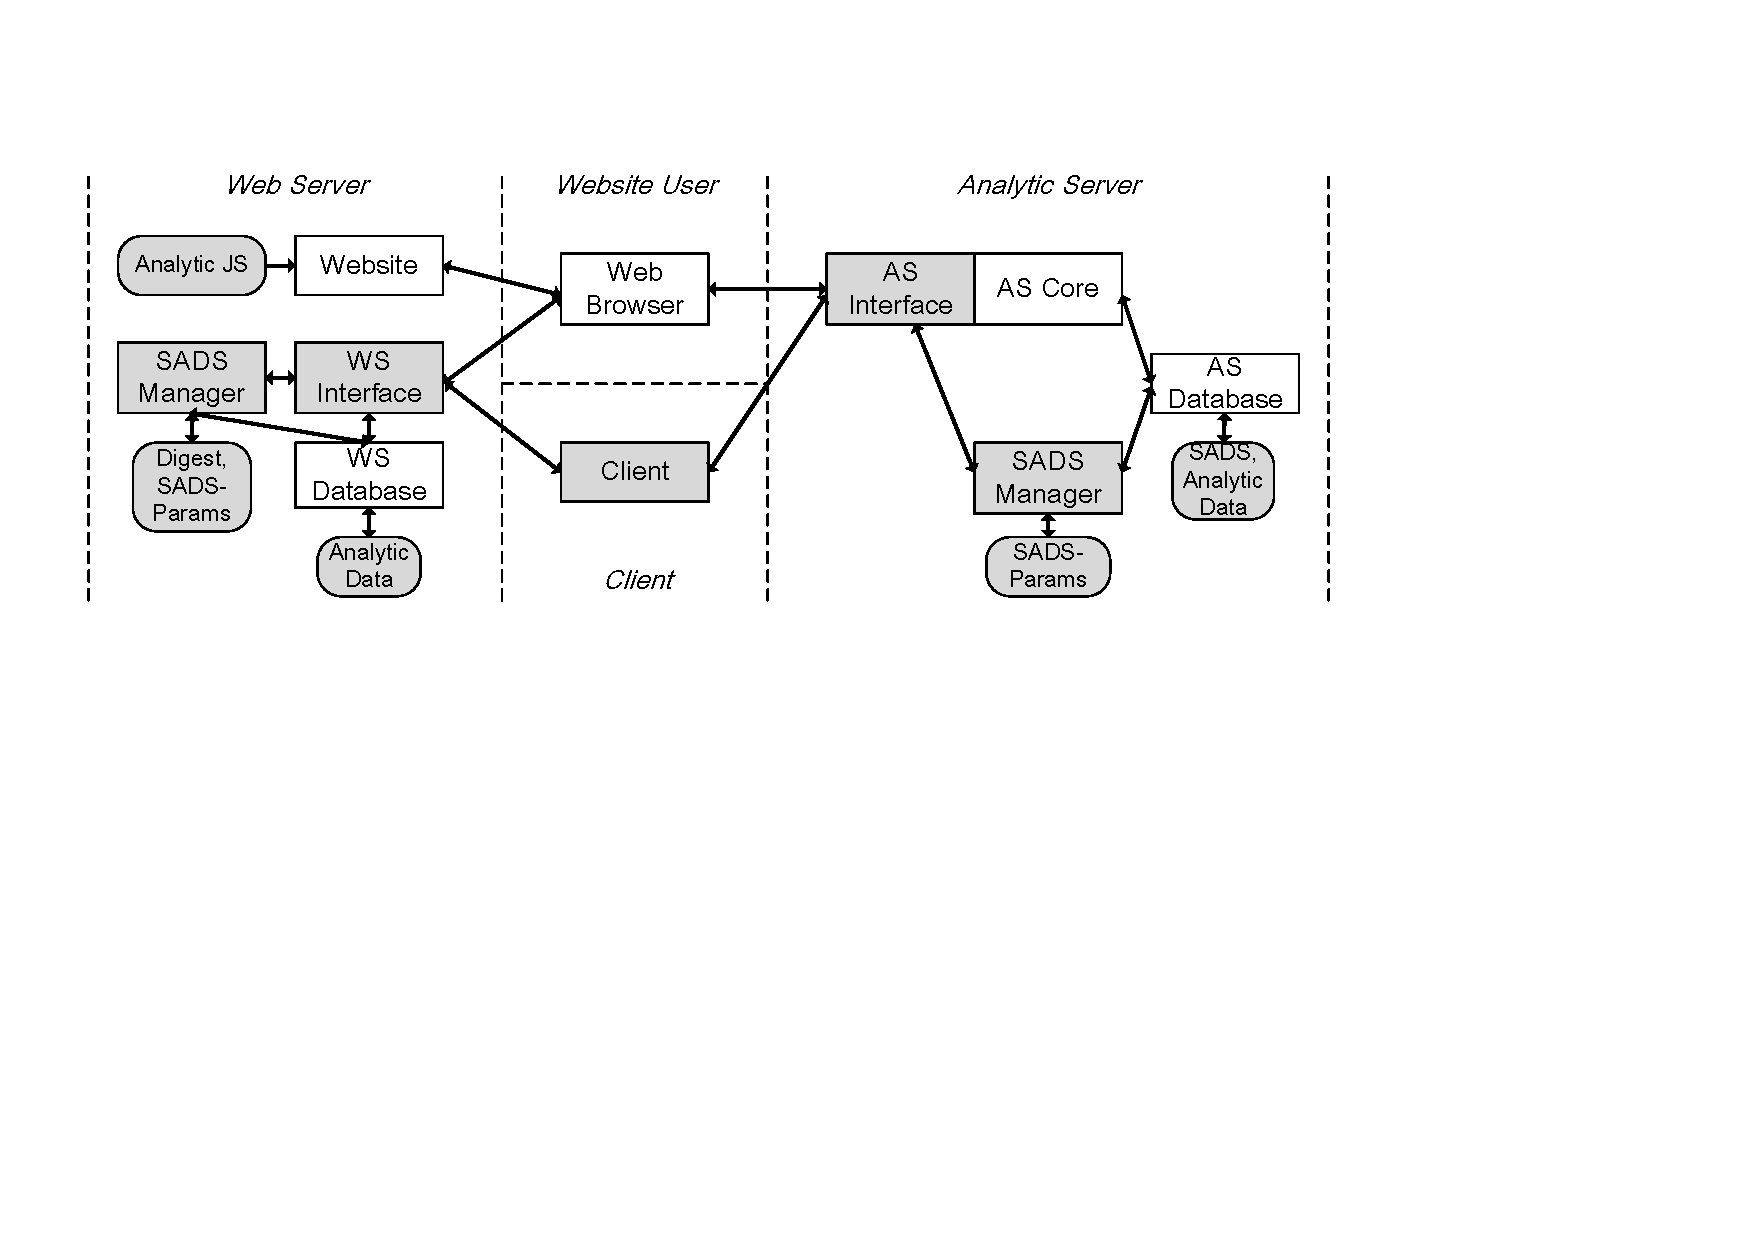
\includegraphics[width=1.0\textwidth]{figure/architecture.pdf}
\caption{Architecture of the project.  Rectangular and rounded boxes represent processes and data, respectively.  Shading indicates components added or modified by the project.}
\label{fig:architecture}
\end{figure}

%%%%%%%%%%%%%%%%%%%%%%%
\subsection{Architecture Overview}
%%%%%%%%%%%%%%%%%%%%%%%
Figure \ref{fig:architecture} shows the components of the project.
Shaded entities are implemented/modified in the project.

\emph{Analytic Server} stores analytic data from user web browsers and manages SADS to prove the correctness of the analytic data. 
Upon receiving analytic data from website user's web browser, the analytic server i) stores the received analytic data in the database and ii) updates the SADS.
Also, the analytic server handles queries from clients. 
When the analytic server receives a query from the client, it responds with the result of the query along with the proof derived from SADS. 

\emph{Web Server} hosts the website of the client where analytic Javascript is embedded.
The web server also deals with analytic data received from website user's web browser and then it builds the digest based on the received analytic data.
The digest is for verifying the proof of the answer of analytic server.

When \emph{Website User} accesses the website using a commodity web browser, and the analytic Javascript is transferred to the web browser along with the website contents.
The web browser collects analytic data by running analytic Javascript and sends the collected analytic data to both analytic server and web server through \emph{2-Phase commit} protocol. 
2-Phase commit protocol is described in \ref{label:2phase_commit}.

\emph{Client} is the owner of the website associated with the analytic server. 
Client sends a query to the analytic server and receives an answer to the query along with the proof. 
Then he verifies the answer and the proof using the digest received from the web server. 
If any inconsistency between the digest of the web server and SADS of the analytic server is found, the client executes \emph{reconcile} protocol to recover the consistency.
Reconcile protocol is described in \ref{label:reconcile}.

%%%%%%%%%%%%%%%%%%%%%%%
% Analytic Server
%%%%%%%%%%%%%%%%%%%%%%%
\subsection{Analytic Server}
\subsubsection{AS Interface}
\label{subsub:as_interface}
The genuine analytic server such as Google Analytics and Piwik consists of \emph{AS Core} and AS interface.
The analytic server provides \emph{AS Interface} for receiving analytic data from web browsers and for handling queries from the client.
AS interface is a part of analytic server program but we logically separate it from the analytic server program to integrate SADS into the original analytic server program. 

Basically, AS interface receives analytic data from the website users' web browsers and forwards to \emph{AS core} which processes the analytic data. 
In addition to this genuine function, AS interface forwards whole (or part of) analytic data to \emph{SADS manager} when it is confirmed that the web server also has received the analytic data. 
AS interface also forwards queries and other messages related to reconciliation process to SADS manager. 

\subsubsection{AS Core}
\emph{AS Core} is a part of the genuine analytic server. 
It processes analytic data and queries from the client. 
In this project, AS core performs its genuine functions and therefore it is not modified. 


\subsubsection{SADS Manager}
\emph{SADS manager} in analytic server maintains SADS-related parameters such as security parameter $k$, matrices $\mathbf{L}$ and $\mathbf{R}$ and other necessary parameters while the whole tree structure for SADS and necessary partial digest table are stored in \emph{Database}. 
It handles analytic data and update SADS stored in the database.
It also processes queries received through AS interface and generates corresponding answers and proofs. 
In addition, it performs reconciliation process when it receives relevant message.
Whenever it updates values of leaf nodes of SADS tree, it should check the log of analytic data stored by AS core so that SADS and stored analytic data are synchronized. 


\subsubsection{AS Database}
AS database maintains log of received analytic data and the table for SADS tree.
Log of analytic data is managed by AS core and it is not modified in this project.

A table for SADS tree consists of two columns, \emph{$<$ID, Value$>$}.
Assuming that the size of the universe $\mathcal{U}$ is $M = 2^m$, the size of \emph{ID} is set to $(M+1)$ bits. 
IDs of leaf nodes are expressed as in the form of $(1 || nodeid)$ where $nodeid$ is $M$-bit string for $2^M$ leaf nodes.
Then the ID of parent node of an arbitrary child node can be set to $(1|| {\lfloor nodeid/2 \rfloor})$.
As an example, if we want to build a SADS tree that stores visiting count per IP address, $33$ bits are necesary for ID of each node since $nodeid$ of a leaf node is 32-bit IP address of a user.

%A table for partial digest consists of three columns, \emph{$<$ID, ID$_{ref}$, Value$>$}.



%%%%%%%%%%%%%%%%%%%%%%%
% web server
%%%%%%%%%%%%%%%%%%%%%%%
\subsection{Web Server}
\subsubsection{WS Interface}
AS interface depicted in \ref{subsub:as_interface} would be reused as \emph{WS interface}.
However, WS interface would need partial functionalities of AS core since it needs to process received analytic data and store it into WS database.

\subsubsection{SADS Manager}
SADS manager in web server also maintains SADS-related parameters, as SADS manager in analytic server does. 
Upon receiving analytic data, SADS manager updates its digest using SADS-related parameters.
When SADS manager receives a request for the digest, it returns its digest to the client.
Also it needs to handle messages related to reconciliation process.


%%%%%%%%%%%%%%%%%%%%%%%
% client
%%%%%%%%%%%%%%%%%%%%%%%
\subsection{Client}
Client sends a query to analytic server and gets an answer and its proof.
Also it requests the digest from web server.
Then client performs verification process to verify if the answer and the proof received from the analytic server match to the digest received from the web server.
If verification fails, the client performs reconciliation process by comparing partial list of analytic data of analytic server and web server. 
Reconciliation process is further described in \ref{label:reconcile}.
